\documentclass[11pt]{article}
% DOC HYBRID MANUSCRIPT: temporal residual learning and integrated station adaptation.
\usepackage[margin=1in]{geometry}
\usepackage[T1]{fontenc}
\usepackage{lmodern,microtype}
\usepackage{amsmath,amssymb,booktabs,array,xcolor,graphicx}
\usepackage{caption,placeins}
\usepackage[numbers,sort&compress]{natbib}
\usepackage{xurl}
\usepackage[hidelinks]{hyperref}
\definecolor{riverblue}{HTML}{235B80}
\definecolor{supportorange}{HTML}{D08043}
\captionsetup{font=small,labelfont=bf}
\setlength{\emergencystretch}{2em}
\title{Reconstructing sparse river dissolved organic carbon with environmental prediction and observation-aware residual learning}
\author{Zhaochen Yang\\[2pt]\small Working manuscript --- October 2026}
\date{}
\begin{document}
\maketitle

\begin{abstract}
Sparse river dissolved organic carbon (DOC) records hinder the analysis of aquatic carbon dynamics. Environmental models provide strong background predictions, while irregular observation histories and differences among stations create additional reconstruction challenges. We propose an integrated framework combining an environmental-context tree predictor, an observation-aware recurrent residual expert, and sparse station adaptation. The recurrent branch learns station-blocked out-of-fold errors of a local tree model; a validation-selected combination integrates the two experts, and local observations adjust target-station predictions. Across a 357-station river cohort and five training seeds, the temporal hybrid reduces MAE from 1.047 to 0.887~mg/L for unobserved periods and from 1.016 to 0.784~mg/L for observation-assisted periods, improvements of 15.3\% and 22.9\% over a selected ExtraTrees context predictor. A further nine-fit experiment across three station partitions shows that five observations per target station reduce hybrid MAE from 2.002 to 1.626~mg/L, an 18.8\% improvement on fixed query cells. The equally calibrated ExtraTrees model achieves 1.609~mg/L, showing that station adaptation, rather than an additional hybrid advantage, accounts for the established spatial benefit. These results connect two practical routes to sparse DOC reconstruction: residual temporal learning for missing periods and local calibration for withheld stations. More transferable expert combination and observation-conditioned temporal adaptation are the next steps toward a unified improvement across both settings.
\end{abstract}
\paragraph{Keywords:} dissolved organic carbon; sparse monitoring; water-quality reconstruction; residual learning; recurrent neural network; spatial adaptation

\section{Introduction}
River dissolved organic carbon connects terrestrial carbon sources with downstream aquatic environments. Its concentration varies with watershed properties, hydrological conditions, and biogeochemical processing, with substantial differences among regions \citep{yang2017}. Reconstructing DOC records can support analysis of long-term carbon dynamics and comparison among catchments. Recent work has demonstrated the value of combining machine learning with environmental and satellite information to recover river organic-carbon patterns over large areas and extended periods \citep{tian2025}. These applications require predictions at locations and times where direct chemical measurements are unavailable.

The observation problem is persistent. Water chemistry is often sampled less continuously and less consistently across sites than meteorology or streamflow, as illustrated by large-sample chemistry compilations \citep{sterle2024}. A river monitoring record can contain isolated gaps, prolonged interruptions, partially observed later periods, and stations with little or no target chemistry. Each case leaves a different set of information available for reconstruction. A nearby measurement may help with a short gap, whereas an unmonitored station must rely more heavily on environmental similarity and observations elsewhere.

Existing methods provide complementary strengths. Temporal interpolation and seasonal summaries offer simple local references when surrounding observations exist. Stream-network geostatistics represent hydrological distance and flow connectivity, extending spatial prediction beyond straight-line proximity \citep{verhoef2006}. Environmental machine learning, including random forests and extremely randomized trees, can represent nonlinear associations among predictors \citep{breiman2001,geurts2006}. Such models can also use manually constructed lags and neighboring-observation summaries; their predictive ability is therefore a demanding baseline for a new temporal method. Recurrent graph models already combine spatial and temporal representations for missing-data reconstruction \citep{cini2022}, while observation-aware recurrent models use missingness masks and elapsed observation time to inform memory updates \citep{che2018}.

The remaining methodological question concerns how these information sources should share the reconstruction task. A strong environmental predictor can explain much of the background variation, leaving errors that may depend on observation history. Asking a neural model to predict the complete DOC signal requires it to relearn that background as well as any remaining dynamics. Conversely, a tree model supplied with a fixed set of lags may not capture all useful relationships in an irregular observation sequence. This motivates a division of prediction into an environmental reference and a temporal correction, followed by a combination that can retain useful information from both.

We propose an integrated DOC reconstruction model that combines environmental prediction, observation-aware residual learning, and sparse station adaptation. A fixed local tree model supplies the reference for a recurrent residual expert, trained on errors from station-blocked out-of-fold predictions. Observation age, recent support, ecological descriptors, and hydroclimatic inputs inform its correction. A separate environmental-context expert uses visible local and river-network summaries, and validation data determine how to combine the two complete predictions. At a new monitoring station, a small set of DOC measurements then adjusts the combined prediction to the station's concentration level. This design connects transferable environmental relationships, temporal information, and local observations in one fitted prediction workflow.

This study makes three contributions. First, we introduce an integrated reconstruction method in which environmental prediction supplies a reference, recurrent learning corrects its residual dynamics, and sparse observations adapt the prediction at a target station. Second, matched component comparisons establish the complementary value of environmental and temporal prediction for prolonged monitoring gaps, using tree baselines that already include observation history and river context. Third, three new station partitions quantify the value of one to five local observations and distinguish station calibration from additional neural prediction gains. Station-level analyses relate these benefits to observation availability, environmental similarity, and flow variability. Together, these contributions explain how environmental relationships, temporal memory, and local observations contribute to different DOC reconstruction tasks.

\section{Materials and methods}

\subsection{River cohort and reconstruction tasks}
We use a Mississippi River basin cohort of 357 stream stations connected by 324 directed river-network edges. The monthly grid spans April 1972 to September 2026, comprising 654 months and 233,478 station-month positions. Only 22,571 positions (9.67\%) contain observed DOC, illustrating the sparsity of the reconstruction problem. The present study focuses on DOC concentration in mg/L. Dynamic covariates are water temperature and discharge with availability indicators. Static inputs describe station location and ecological regime. DOC targets are transformed as $z=\log(1+y)$, where $y$ denotes concentration.

The original four evaluation scenarios represent different monitoring gaps (Table~\ref{tab:scenarios}). Random gaps withhold observed station-month cells. Unobserved periods withhold target observations in a later time segment. Observation-assisted periods retain designated observations as context in that segment. Unmonitored stations withhold the target record at a group of stations. This experiment uses one existing split per scenario and five training seeds, 42--46. A second experiment, described below, evaluates integrated station adaptation across three new station partitions. Splits are held constant across the compared methods. Spatially and temporally structured evaluation follows the principle of matching a split to its intended prediction setting \citep{roberts2017}.

\begin{table}[htbp]\centering\small
\caption{Evaluation tasks. Counts are unique query cells and contributing stations within each scenario. The same cells can occur in different scenarios.}
\label{tab:scenarios}
% BEGIN GENERATED SCENARIOS
\begin{tabular}{>{\raggedright\arraybackslash}p{4.3cm}rr}\toprule
Scenario & Query cells & Stations\\\midrule
Random gaps & 4,514 & 355\\
Unobserved periods & 2,223 & 69\\
Observation-assisted periods & 1,778 & 67\\
Unmonitored stations & 2,531 & 43\\
\bottomrule\end{tabular}
% END GENERATED SCENARIOS
\end{table}

In the original four-scenario experiment, model fitting and validation inference use only training and designated context observations as target inputs. Validation labels enter early stopping and model combination, but not the input features. Terminal inference additionally permits validation observations as context; the evaluated query labels remain hidden. The new station-partition experiment retains training-only target inputs at both validation and test inference. Current hydrological covariates are assumed available in both experiments. The task is reconstruction of missing DOC under specified information availability.

\subsection{An environmental-context predictor}
The context predictor $C_{it}$ uses 39 features for station $i$ and month $t$: temperature and discharge with their visibility flags, seasonal sine/cosine terms, coordinates, 13 regime descriptors, six visible-DOC context summaries, and 12 local lag features. The context summaries contain global, upstream, and downstream visible DOC means and support fractions. Means are calculated in log-transformed target space and exclude the query cell. The local lags describe observations at one, three, six, and twelve months, including availability.

All context forests contain 300 trees. In the original four-scenario experiment, validation MAE selects among six candidates for each seed and scenario: random forests with minimum leaf sizes one or two, and ExtraTrees variants using all-feature or square-root-feature split selection and minimum leaf sizes one, two, or four. All selected context experts are ExtraTrees: leaf size four in the temporal scenarios, leaf size two for random gaps, and leaf sizes one or two for unmonitored stations. A fixed 300-tree random forest with leaf size one is retained as an additional baseline on the same features, seeds, and query cells.

This predictor already uses explicit temporal and river-context information. Its comparison with the hybrid therefore measures the added value of the learned residual expert and combination, beyond an environmental model that already has engineered history and neighborhood features.

\subsection{An observation-aware temporal residual expert}
\subsubsection{Local reference and out-of-fold residual targets}
A separate local forest defines the reference for residual learning. It is an ExtraTrees model with 300 trees, minimum leaf size four, and all features available at each split. Its 40 predictors retain environmental and lag information but replace the six network-context columns with seven strictly historical local features: the most recent value, log observation age, an availability flag, and observation counts over the preceding one, three, six, and twelve months. This local reference $B$ is distinct from the selected context expert $C$.

We partition training stations into five folds. For each fold, the local forest is fitted on the other four folds, and all target observations at the withheld stations, including context observations, are hidden from its input construction. Let $B_{it}^{\mathrm{OOF}}$ be the resulting prediction in log space. The neural target is
\begin{equation}
 r_{it}^{\mathrm{OOF}}=\frac{z_{it}-B_{it}^{\mathrm{OOF}}}{\sigma_{\mathrm{train}}},
 \label{eq:oof}
\end{equation}
where $\sigma_{\mathrm{train}}$ is the standard deviation of transformed training labels. The neural branch uses the corresponding fold-specific observation view. This construction gives the branch an error signal from station withholding rather than residuals from an in-sample forest fit.

\subsubsection{Observation-aware memory}
The neural branch combines a two-layer ecological encoder with a two-layer, 64-unit node encoder. The ecological encoder maps nine regime variables through two 32-unit layers. Monthly node inputs contain hydroclimatic values and masks, season, location, visible DOC and its availability, hydro-regime descriptors, and observation-support features. The latter include the last visible value, log age, an ever-observed flag, support fractions at four time scales, and upstream support. Downstream support is zero in the selected residual configuration.

For each prediction month, a 12-month window is processed by an observation-aware GRU with 64 hidden units. Inspired by observation-decay approaches \citep{che2018}, the hidden state is attenuated before its recurrent update:
\begin{align}
 \gamma_{it}&=\exp\{-\operatorname{ReLU}(W_d q_{it}+b_d)\},\\
 h_{it}&=\operatorname{GRUCell}([e_{it},v_t],\,\gamma_{it}\odot h_{i,t-1}),
\end{align}
where $e_{it}$ is the encoded monthly state, $v_t$ indicates valid history, and $q_{it}$ contains scaled log observation age, an observation-availability indicator, upstream support, and a zero downstream-support channel. Each window starts from zero recurrent state, and padded positions make no recurrent update. Input windows end at the prediction month. Visible observations at the current month may enter support features; hidden query values cannot.

The residual expert uses a self-node encoder without learned edge messages or an attention operator. River connectivity enters through explicit observation-support features. Separate message and lag-attention controls examine the potential additional value of learned river propagation.

\subsubsection{Residual prediction and training}
A zero-initialized scalar head maps the final hidden state to a standardized residual $d_{\theta,it}$. Using a local forest refitted on all training cells, the complete residual-expert prediction is
\begin{equation}
 R_{it}=\max\{0,\exp(B_{it}+\sigma_{\mathrm{train}}d_{\theta,it})-1\}.
 \label{eq:residual}
\end{equation}
At initialization, the correction is zero and this expert equals its local reference, $B^y_{it}=\max\{0,\exp(B_{it})-1\}$ in concentration units. The forest is fixed throughout neural training.

Training minimizes mean squared error on the standardized out-of-fold residuals. Five station folds contribute to one accumulated optimizer step per epoch. We use Adam with learning rate $10^{-3}$, gradient-norm clipping at one, dropout 0.1, at most 20 epochs, and early-stopping patience five. Completed temporal runs stop after 15--16 epochs. Early stopping evaluates the complete local-reference-plus-residual prediction. Target and dynamic-input scaling are based on training cells; static descriptor scaling uses the known station cohort. The prediction applies a lower bound of zero after inverse transformation, with no upper-quantile clipping.

\subsection{Combining the two complete experts}
For temporal scenarios and the new station-partition experiment, the candidate outputs are context-only, residual-expert-only, a geometric blend, and a log-affine combination. The latter is
\begin{align}
 \hat z_{it}&=\beta_0+\beta_C\log(1+C_{it})+\beta_R\log(1+R_{it}),\\
 H_{it}&=\max\{0,\exp(\hat z_{it})-1\}.
 \label{eq:fusion}
\end{align}
Unconstrained least squares fits the affine coefficients on validation predictions. The geometric-blend weight is selected on a grid with step 0.005. Raw-scale validation MAE selects the candidate output. All ten temporal seed--scenario combinations select the affine form. Its weights combine complete expert predictions and are neither attention weights nor physical coefficients.

Random gaps and the original unmonitored-station task use the context expert directly under the existing scenario-specific configuration. Their final outputs therefore equal the context baseline. The new station-partition experiment applies validation selection to the spatial task as well, then calibrates the selected predictor using sparse observations at each target station. Figure~\ref{fig:architecture} shows the integrated prediction workflow.

\begin{figure}[htbp]\centering
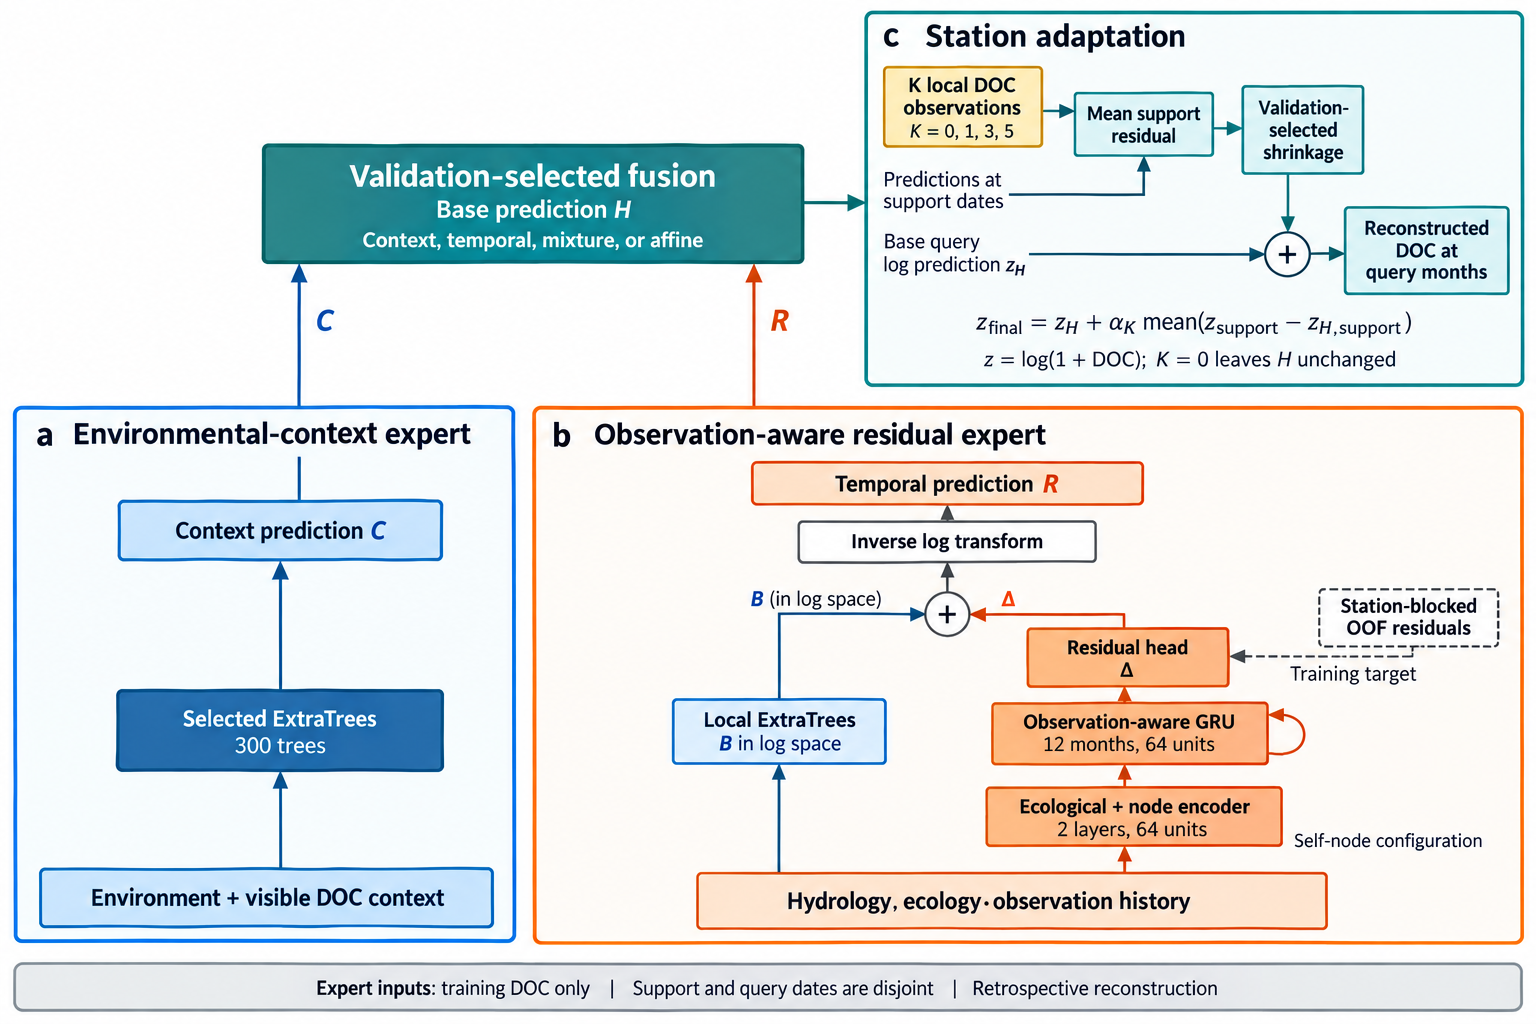
\includegraphics[width=\linewidth,height=.65\textheight,keepaspectratio]{figures/doc_unified_architecture_v2.png}
\caption{\textbf{An integrated model for DOC reconstruction and station adaptation.} \textbf{a,} An environmental-context expert supplies prediction $C$. \textbf{b,} A recurrent branch learns station-blocked out-of-fold residuals of the separate local reference $B$, producing the complete temporal expert $R$. Validation selection combines the two complete predictions into $H$. \textbf{c,} Sparse observations provide a station-specific correction in log space, followed by inverse transformation and a lower bound of zero. The experts remain fixed during station adaptation. Dashed arrows show training supervision. The training-only input rule shown here applies to the new station-partition experiment; the original temporal experiment uses its designated context views.}
\label{fig:architecture}
\end{figure}

\subsection{Integrated adaptation at withheld stations}
The new spatial experiment evaluates the environmental and temporal experts together with station calibration. Three random station partitions of the same 357-station cohort each contain 232 training, 54 validation, and 71 test stations. Partition seeds are 142--144, with training seeds 42--44 within each partition. These partitions assess transfer of DOC prediction to withheld monitoring stations while the station covariates and river network remain available. They introduce new label-withholding tasks within the development cohort.

Both experts receive training-station DOC only during validation and test inference. Validation observations guide early stopping, environmental-expert selection, fusion, and calibration strength. For this experiment, the context expert is selected from four 300-tree ExtraTrees configurations: minimum leaf sizes four, two, and one using all features, and leaf size one using square-root feature selection. The temporal expert retains the architecture and training budget above. A context-only fusion candidate remains available, and its selection is recorded for each fit.

At each target station, five observed dates are reserved in the order first, middle, last, first quartile, and third quartile of the observed record. Nested prefixes define $K=0,1,3,5$ support budgets. All five candidates are excluded from evaluation at every budget. The three partitions contain 3,975, 3,907, and 4,983 fixed query cells, respectively. Support dates can follow query dates, so the task is retrospective record reconstruction.

For a predictor $P\in\{C,H\}$ and support set $\mathcal S_i^{(K)}$, the station correction is
\begin{align}
 \bar r_{i,P}^{(K)}&=\frac{1}{K}\sum_{s\in\mathcal S_i^{(K)}}
       [\log(1+y_{is})-\log(1+P_{is})],\\
 \widehat y_{it,P}^{(K)}&=\max\{0,\exp[\log(1+P_{it})+
                      \alpha_{P,K}\bar r_{i,P}^{(K)}]-1\}.
 \label{eq:station_adaptation}
\end{align}
For $K=0$, the original prediction is returned unchanged. The support residual compares observed and predicted DOC at the same dates. Source-validation tasks select $\alpha_{P,K}$ separately for each predictor and budget from $\{0,0.25,0.5,0.75,1\}$ using raw-scale MAE. Support observations enter this output correction; they do not update the experts' inputs, recurrent states, or fitted weights.

Four matched arms separate the contributions of the hybrid and local observations: ExtraTrees, calibrated ExtraTrees, the hybrid, and the calibrated hybrid. The principal comparison is calibrated hybrid versus calibrated ExtraTrees at $K=5$. The $K=0$ comparison and each model's change from $K=0$ to $K=5$ distinguish expert combination from station calibration. Two supplementary controls examine the source of the hybrid gain. A context-only affine recalibration tests the value of the second expert beyond a global adjustment of the context prediction's scale. A combination of $C$ and the uncorrected local forest prediction $B^y$ uses the same validation-selected fusion and calibration, testing the added predictive contribution of the learned residual in $R$. Each control independently selects its coefficients on the same validation tasks. These diagnostic comparisons were added after the first formal run; they do not replace the four primary arms.

Metrics average the three seed results within each partition, then weight the three partitions equally. Paired intervals resample station identities jointly across partitions 5,000 times. A station appearing in multiple partitions receives the same bootstrap multiplicity in each; all its query cells contribute within each partition. This preserves both the cell-weighted error and dependence due to repeated stations. Station-level changes describe variation in the adaptation benefit. Descriptive stratification uses environmental novelty, visible upstream support, DOC record availability, and discharge variability. Record availability counts observed DOC months; every station still receives the same support budget $K$. Discharge variability is the coefficient of variation over available monthly flow observations, requiring at least 12 months and positive mean flow. Record-availability and flow-variability groups use training-station tertiles within each partition.

\subsection{Evaluation and component comparisons}
Primary performance is MAE on hidden DOC cells. RMSE, $R^2$, log-space MAE, and training-derived Q90 tail MAE provide complementary summaries. In the original four-scenario experiment, reported metrics average the five individual seed metrics; the station-partition experiment uses the three-seed and three-partition aggregation described above. These are averages of individual-model errors. Table~\ref{tab:main} compares the fixed random-forest context model, validation-selected ExtraTrees context model, and final hybrid. In temporal scenarios, the complete residual expert is additionally compared on identical query cells.

For paired intervals, absolute errors are averaged across seeds at each cell, then whole stations are resampled 5,000 times. Each sampled station contributes all query cells, preserving the main cell-weighted estimand within each replicate. Intervals are reported for the hybrid-minus-context MAE difference and relative reduction. Seed variation is summarized separately. Q90 groups with fewer than 20 distinct cells are marked as small-sample diagnostics.

The earlier regional extension (Appendix~\ref{app:regional}) uses the same paired station-resampling principle. A descriptive station-shuffle diagnostic assigns fitted corrections to different target stations, using one fixed permutation per seed and support budget. Model development has repeatedly used the original four scenario splits. The new station-partition experiment evaluates the integrated prediction workflow across three additional label-withholding tasks; an independent river basin remains a next test of geographical generalization.

\FloatBarrier
\section{Results}

\subsection{The hybrid improves reconstruction across unobserved periods}
The environmental-context predictor is a strong baseline across all four scenarios (Table~\ref{tab:main}). Combining it with the temporal residual expert reduces MAE from 1.047 to 0.887~mg/L in unobserved periods and from 1.016 to 0.784~mg/L in observation-assisted periods. These changes correspond to improvements of 15.3\% and 22.9\%, respectively. Both temporal scenarios improve across all five seeds.

The station-resampled 95\% interval for the MAE difference is $[-0.262,-0.050]$~mg/L in unobserved periods and $[-0.307,-0.159]$~mg/L in observation-assisted periods. Corresponding relative-improvement intervals are 4.7--25.0\% and 17.2--27.9\% (Figure~\ref{fig:performance}). The gains therefore persist when stations are resampled within each existing split.

\begin{table}[htbp]\centering\small
\caption{Five-seed reconstruction performance. MAE and RMSE are in mg/L. The hybrid equals the ExtraTrees context route in random gaps and unmonitored stations.}
\label{tab:main}
% BEGIN GENERATED MAIN RESULTS
\setlength{\tabcolsep}{4pt}
\begin{tabular}{>{\raggedright\arraybackslash}p{3.5cm}rrrrr}\toprule
Scenario & \shortstack{RF\\MAE} & \shortstack{ET\\MAE} & \shortstack{Hybrid\\MAE} & \shortstack{Hybrid\\RMSE} & \shortstack{Hybrid\\$R^2$}\\\midrule
Random gaps & 1.452 & 1.436 & 1.436 & 6.626 & 0.384\\
Unobserved periods & 1.070 & 1.047 & 0.887 & 1.404 & 0.470\\
Observation-assisted periods & 1.051 & 1.016 & 0.784 & 1.228 & 0.587\\
Unmonitored stations & 2.687 & 2.545 & 2.545 & 5.330 & 0.455\\
\bottomrule\end{tabular}
% END GENERATED MAIN RESULTS
\end{table}

\begin{figure}[htbp]\centering
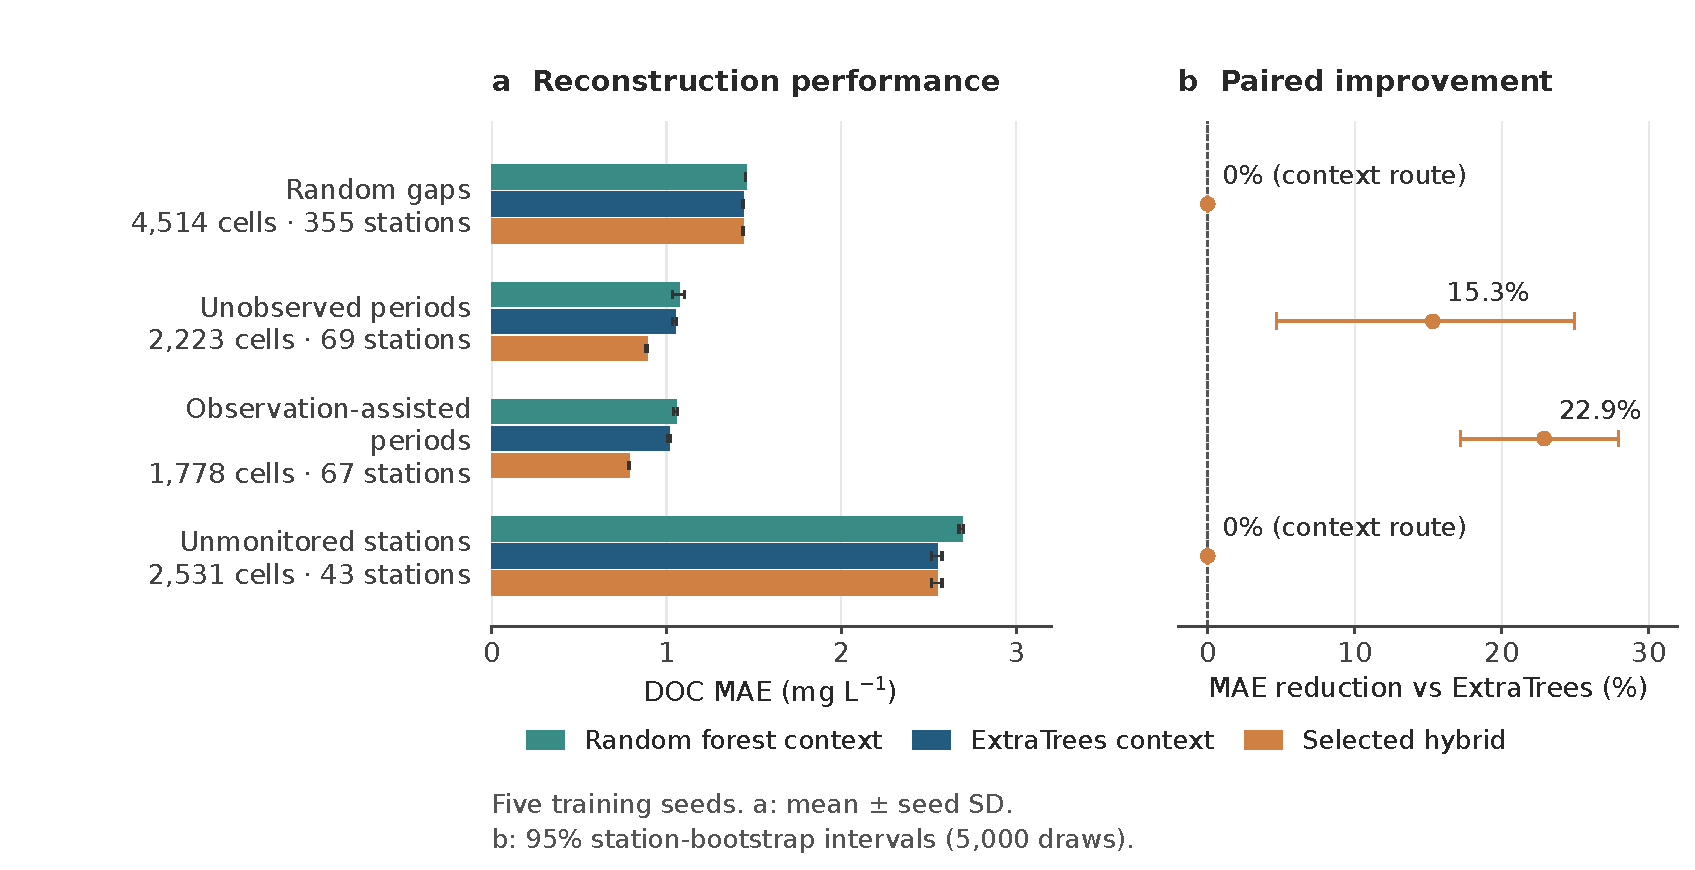
\includegraphics[width=\linewidth]{figures/doc_hybrid_performance.pdf}
\caption{\textbf{Performance by monitoring gap.} \textbf{a}, Mean individual-seed MAE for matched context baselines and the hybrid; error bars show seed SD. \textbf{b}, Relative improvement over selected ExtraTrees with paired station-bootstrap 95\% intervals. Zero gain in random gaps and unmonitored stations reflects the context-only route. Counts refer to unique query cells within each scenario.}
\label{fig:performance}
\end{figure}

Random-gap MAE is 1.436~mg/L and unmonitored-station MAE is 2.545~mg/L, identical to the context expert by construction. These cases establish the retained baseline performance of the deployed configuration, rather than an increment from neural correction. Averaging losses across all scenario-cell occurrences gives hybrid MAE 1.475~mg/L, compared with 1.545 for ExtraTrees and 1.593 for the fixed random forest. The 11,046 scenario-cell occurrences include 8,150 distinct cells because scenarios overlap; this pooled summary is descriptive, and the scenario-specific comparisons carry the main inference.

\subsection{The two complete experts supply complementary predictions}
The learned correction improves its matched local reference in both temporal scenarios (Table~\ref{tab:components}). In unobserved periods, MAE decreases from 1.148~mg/L for the local forest to 0.946 for the complete residual expert, a 17.6\% reduction. In observation-assisted periods, it decreases from 0.973 to 0.795~mg/L, an 18.3\% reduction. All five seeds improve in each comparison. This directly establishes the added value of the trained neural residual branch relative to its own base.

The complete residual expert also outperforms context ExtraTrees, whose MAEs are 1.047 and 1.016~mg/L. Affine fusion further reduces error to 0.887 and 0.784~mg/L, gains of 6.2\% and 1.4\% relative to the complete residual expert. All five seeds favor fusion in each comparison.

\begin{table}[htbp]\centering\small
\caption{Matched temporal component comparison. The local base is the forest corrected by the neural branch; the context expert is a separate forest. The complete residual expert includes its local base and correction. Values are mean individual-seed MAEs on identical query cells.}
\label{tab:components}
% BEGIN GENERATED COMPONENTS
\begin{tabular}{>{\raggedright\arraybackslash}p{3.7cm}rrrr}\toprule
Scenario & Local base & Context & Residual expert & Hybrid\\\midrule
Unobserved periods & 1.148 & 1.047 & 0.946 & 0.887\\
Observation-assisted periods & 0.973 & 1.016 & 0.795 & 0.784\\
\bottomrule\end{tabular}
% END GENERATED COMPONENTS
\end{table}

\begin{samepage}
This sequence supports the complementary roles of the two complete predictors: the recurrent correction improves its local reference, and the environmental-context expert supplies additional information that improves their combined prediction. Earlier matched river-message and lag-attention controls gave little additional DOC improvement over self-node residual models, motivating the selected configuration. The temporal performance gain is consequently attributed to the evaluated residual-expert combination.
\par\end{samepage}

\subsection{Sparse local observations improve reconstruction at withheld stations}
The integrated spatial experiment completed all nine partition--seed fits. Its three partitions contain 172 distinct test stations and 10,520 distinct query cells, represented by 213 station--partition cases and 12,865 query-cell occurrences. All nine fits select log-affine expert combination. With five support observations per station, hybrid MAE decreases from 2.002 to 1.626~mg/L, an 18.8\% reduction (95\% interval 13.8--23.7\%; Table~\ref{tab:unified}; Figure~\ref{fig:unified}). All three partitions and all nine fitted replicates improve. Three observations already reduce MAE to 1.675~mg/L; one observation yields a smaller change to 1.943~mg/L.

\begin{table}[htbp]\centering\small
\caption{Integrated reconstruction on the three new station partitions. Metrics average three training seeds within each partition and then weight partitions equally. The query is fixed across all four arms and observation budgets. Concentration errors are in mg/L.}
\label{tab:unified}
\begin{tabular}{lrrrrr}\toprule
Predictor & $K$ & MAE & RMSE & $R^2$ & Q90 MAE\\\midrule
ExtraTrees & 0 & 1.903 & 4.008 & 0.467 & 7.559\\
Hybrid & 0 & 2.002 & 4.122 & 0.433 & 7.823\\
ExtraTrees + calibration & 5 & 1.609 & 3.615 & 0.562 & 6.744\\
Hybrid + calibration & 5 & 1.626 & 3.593 & 0.567 & 6.607\\
\bottomrule\end{tabular}
\end{table}

\begin{figure}[htbp]\centering
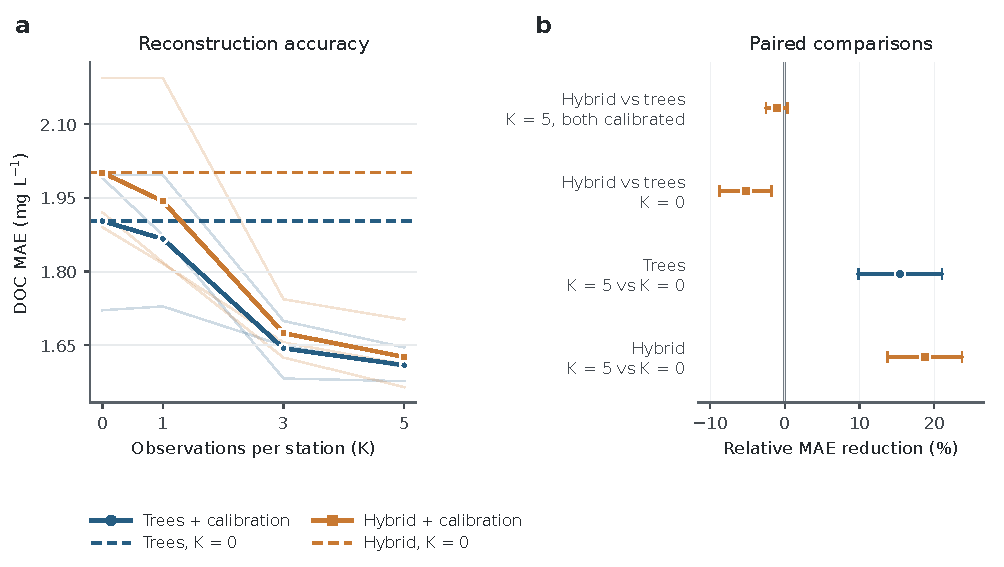
\includegraphics[width=\linewidth]{figures/unified_doc_spatial_main.pdf}
\caption{\textbf{Integrated DOC reconstruction with sparse station calibration.} \textbf{a,} Calibrated ExtraTrees and hybrid MAE as the number of target-station observations increases. Dashed lines show each predictor's uncalibrated reference; pale lines show the three partition trajectories. Bold lines average seeds within partitions, then weight partitions equally. \textbf{b,} Paired relative MAE reductions with 95\% intervals from 5,000 joint station-bootstrap resamples. Positive values favor the first predictor or $K=5$; negative values indicate higher MAE. Each partition contains 71 test stations and three training seeds, with 3,975, 3,907, and 4,983 fixed query cells. There are 172 distinct test stations across partitions. Support dates may follow query dates, consistent with retrospective reconstruction.}
\label{fig:unified}
\end{figure}

The same local observations also improve ExtraTrees, from 1.903 to 1.609~mg/L, a 15.4\% reduction (95\% interval 9.8--21.0\%). The calibrated hybrid has 1.0\% higher MAE than calibrated ExtraTrees; its paired difference is 0.017~mg/L (95\% interval $[-0.005,0.041]$). Without support, hybrid MAE is 5.2\% higher, with a paired difference of 0.099~mg/L ($[0.033,0.172]$). Only one of the three partitions favors the hybrid over ExtraTrees at either endpoint. Thus, sparse calibration transfers successfully across the station partitions, while the temporal hybrid's additional spatial advantage is not established.

\subsection{Component controls locate the remaining spatial challenge}
Context-only affine recalibration produces MAE of 1.983~mg/L without support and 1.629~mg/L at $K=5$. Both are close to the hybrid's corresponding outputs, and paired intervals for hybrid-minus-affine-context differences span zero. Affine recalibration itself increases zero-support ExtraTrees error by 4.2\%. This shared pattern points to transfer of the validation-fitted output adjustment as an important component to improve.

Replacing the corrected temporal expert $R$ with its uncorrected local forest $B^y$ provides a second diagnostic. The resulting two-forest combination has MAE of 2.010~mg/L at $K=0$ and 1.623~mg/L at $K=5$. Adding the recurrent correction gives a small 0.4\% benefit without support (95\% interval 0.12--0.71\%) and a 0.18\% increase in error after calibration (0.03--0.33\%). These effects are much smaller than the benefit of station observations and change direction with the support budget. The controls identify a useful distinction: the recurrent residual supplies substantial information in the original temporal tasks, but its incremental value after expert combination is small in the new station-transfer tasks.

\subsection{Station adaptation benefits vary across environmental settings}
Five-observation calibration improves the hybrid in 162 of 213 station--partition cases, with a median station-level MAE reduction of 6.8\% (Appendix~\ref{app:station_responses}). The corresponding values for ExtraTrees are 150 cases and 5.8\%. Station-level medians are smaller than the overall cell-weighted reductions, reflecting variation in both the size of the benefit and record length.

The hybrid's calibration benefit appears across all three ecological-novelty groups, with descriptive MAE reductions of 11.5\%, 22.0\%, and 21.4\% from lower to higher novelty. It also appears across lower, middle, and higher discharge variability (21.6\%, 14.1\%, and 18.0\%) and DOC record availability (18.9\%, 13.8\%, and 20.8\%). These patterns show broad use of local concentration information, rather than a benefit confined to the densest monitoring records. At the same $K=5$, hybrid MAE remains slightly above calibrated ExtraTrees in all three novelty and discharge-variability groups. The lowest record-availability group shows a small descriptive hybrid advantage of 0.8\%; these strata do not establish a distinct hydrological mechanism.

\subsection{Overall accuracy and high-concentration performance differ}
Improvements in temporal MAE are accompanied by higher $R^2$: from 0.384 to 0.470 in unobserved periods and from 0.428 to 0.587 in observation-assisted periods. RMSE decreases from 1.514 to 1.404~mg/L and from 1.446 to 1.228~mg/L, respectively. These changes extend the temporal gain beyond one loss metric.

High-concentration errors show a different pattern (Appendix~\ref{app:tail}). The two temporal Q90 groups contain only 12 and seven distinct query cells. The hybrid changes tail MAE from 6.759 to 6.712~mg/L in unobserved periods and from 6.862 to 7.129~mg/L in observation-assisted periods. These small groups do not establish improved extreme-value reconstruction. For random gaps, selected ExtraTrees improves MAE slightly over the fixed random forest but has higher RMSE (6.626 versus 6.287~mg/L), further illustrating the importance of reporting more than average absolute error.

The new station partitions contain 352, 440, and 558 Q90 query cells at training-derived thresholds of approximately 9.85, 10.00, and 10.00~mg/L. Calibrated hybrid tail MAE is 6.607~mg/L compared with 6.744 for calibrated ExtraTrees, and its RMSE is also slightly lower (Table~\ref{tab:unified}). These descriptive differences complement the primary MAE comparison; the present paired inference does not separately establish a tail-error improvement.

\FloatBarrier
\section{Discussion}
\subsection{Environmental prediction and temporal correction address different parts of the task}
The results support a practical division of labor in sparse DOC reconstruction. An environmental-context forest supplies a strong reference using nonlinear environmental relationships and engineered observation summaries. The recurrent residual expert is trained to address errors left by a local environmental prediction. Fusing their complete outputs improves temporal reconstruction beyond either expert alone.

This design gives residual learning a specific role. Instead of requiring the recurrent network to estimate every part of DOC variation, the local forest anchors its prediction and the neural branch learns a correction. The out-of-fold construction makes this correction depend on errors at withheld training stations, reducing reliance on the forest's fitted training residuals. Observation-aware memory provides a way to encode the changing availability of historical information. Our component comparison establishes complementarity at the expert level; it does not yet isolate whether elapsed observation time, ecological encoding, or recurrent state contributes most to that complementarity.

The methodological contribution is the organization and training of these complementary tasks for sparse DOC reconstruction. Tree ensembles, recurrent memory, observation decay, and residual modeling each have precedents. Their integration here is evaluated against tree models that already receive explicit lags and river-context features, making the observed temporal improvement a substantive prediction comparison rather than a consequence of withholding history from the baseline.

\subsection{Different monitoring gaps call for different information}
A station with a missing later record and a station with no target history present different learning problems. In the former, observations and hydroclimatic covariates can inform a time-dependent correction. In the latter, the model must transfer relationships across stations with different concentration levels and environmental conditions. The integrated experiment now evaluates temporal residual prediction and station adaptation within the same fitted workflow, exposing the distinct roles of these components.

Sparse local observations improve reconstruction across every station partition for both predictors. Their strongest established contribution is to adjust the target station's concentration reference. The additional hybrid benefit seen in temporal tasks does not carry over to this spatial comparison: the hybrid is worse without target observations and close to calibrated ExtraTrees with five observations. Affine-context and two-forest controls show that a large part of the spatial behavior can arise from output combination and calibration. This directs model development toward transferable expert combination and support-conditioned residual learning. Shrinking validation-fitted output adjustments toward the environmental reference and allowing local observations to inform recurrent states are concrete next steps.

\subsection{Extending the framework with river transport}
River-network geostatistics and graph imputation methods provide established ways to exploit relational structure \citep{verhoef2006,cini2022}. Explicit river-context summaries provide a strong source of spatial information in our context predictor. The earlier local-base message and lag-attention variants produced little additional improvement over their matched self-node residual controls. Their incremental value relative to the final selected context expert remains to be established.

A next step is to enrich the residual branch with flow-conditioned travel times, source--sink states, and observations along connected reaches. These additions would allow the model to represent how information moves through the river network as hydrological conditions change. Suitable flow, volume, and source information would also make it possible to test process constraints on transported loads. The residual formulation provides a direct way to evaluate these developments: each transport component can be tested for the additional information it supplies beyond the environmental reference and explicit river context.

\subsection{Future research directions}
The framework opens four connected directions for extending sparse DOC reconstruction. The first is transfer across regions and river basins. Environmental similarity and a small number of target observations provide a starting point for adapting the model to different catchment settings. Geographically contiguous holdouts and an independent basin would extend the station-partition experiment to larger environmental shifts. These studies could identify which environmental relationships and temporal corrections transfer across regions and where local adaptation adds the most value.

The second direction is event-sensitive reconstruction. Higher-frequency DOC observations paired with rainfall and discharge would support learning of concentration changes during hydrological events. Event-weighted training and tail-focused objectives could then be compared for their ability to recover peak magnitude, timing, and duration. This development would connect the present monthly reconstruction to observed short-term carbon dynamics and provide a richer basis for evaluating high-concentration behavior.

The third direction is adaptation that evolves as monitoring accumulates. The integrated model currently uses sparse local observations to update its station-level prediction reference. Future versions could also update recurrent states and residual dynamics, allowing newly observed DOC to inform subsequent seasonal and event responses. Comparing retrospective calibration with adaptation using only observations available before each prediction would connect the present reconstruction workflow to operational monitoring.

The fourth direction is uncertainty-aware river carbon assessment. Prediction intervals should be developed for the hybrid and evaluated jointly for coverage, width, and high-concentration performance. Combining reconstructed concentrations with discharge at a matching time scale would then support DOC-load estimation, with concentration and flow uncertainty propagated into the resulting loads. This would extend the framework from filling monitoring gaps toward quantifying carbon transport through river networks.

\section{Conclusion}
We developed and evaluated an environmental-context and observation-aware residual framework for sparse river DOC reconstruction. On the existing temporal holdouts, combining the two complete experts reduces MAE by 15.3\% and 22.9\% relative to selected ExtraTrees context predictions, with further improvement over the residual expert alone. These results show that a strong environmental reference and learned residual dynamics can supply complementary predictive information.

The integrated station-transfer experiment shows that five target observations reduce hybrid error by 18.8\% across three station partitions. Equally calibrated ExtraTrees remains slightly more accurate in MAE, identifying station adaptation as the established spatial benefit and expert-combination transfer as the next modeling priority. The resulting framework connects environmental prediction, temporal correction, and sparse monitoring updates in one usable reconstruction model. Extending how local observations inform residual dynamics offers a direct path toward stronger spatial transfer and event-sensitive river carbon assessment.

\section*{Data, code, and figure availability}
The current manuscript is supported by local prediction products and reproducible analysis scripts. The original temporal results are recomputed by \path{analyze_doc_hybrid_manuscript.py}. The integrated station experiment is analyzed by \path{analyze_unified_doc_spatial.py}, with supplementary controls in \path{analyze_unified_doc_affine_control.py} and hydrological stratification in \path{analyze_unified_doc_flow.py}. Publication figures are generated by \path{plot_unified_doc_manuscript.py}. Each fitted model saves the environmental forests, recurrent weights, selected expert combination, and station-calibration parameters, and exposes a shared query/support prediction interface. Earlier regional results remain reproducible with \path{analyze_spatial_manuscript_evidence.py}. A public data and code release has not yet been assigned a persistent identifier. Figure~\ref{fig:architecture} is an AI-assisted architecture schematic checked against the implemented model. All empirical plots are generated from saved numerical predictions.

\appendix
\section{Tail diagnostics and implementation details}\label{app:tail}
Table~\ref{tab:tail} records the high-concentration comparison without treating repeated predictions across seeds as additional observations. Thresholds are estimated from training labels separately for each scenario.

\begin{table}[htbp]\centering\small
\caption{Training-derived Q90 tail MAE (mg/L). Asterisks indicate fewer than 20 unique query cells.}
\label{tab:tail}
% BEGIN GENERATED TAIL RESULTS
\begin{tabular}{>{\raggedright\arraybackslash}p{3.8cm}rrrr}\toprule
Scenario & Threshold & Cells & ET MAE & Hybrid MAE\\\midrule
Random gaps & 10.00 & 431 & 6.748 & 6.748\\
Unobserved periods & 11.00 & 12* & 6.759 & 6.712\\
Observation-assisted periods & 11.00 & 7* & 6.862 & 7.129\\
Unmonitored stations & 9.40 & 510 & 6.906 & 6.906\\
\bottomrule\end{tabular}
% END GENERATED TAIL RESULTS
\end{table}

The temporal expert uses nine ecological encoder inputs, 14 base monthly channels, and nine observation-aware channels before ecological embedding. The node representation has width 64 and the ecological embedding width 32. The self-node encoder is inherited from the graph implementation; excluding edge messages leaves the node transformation and explicit upstream-support feature intact. Residual targets, input visibility, and the terminal expert combination are defined by Equations~\ref{eq:oof}--\ref{eq:fusion}. Reproduction should use the selected product settings described here, rather than earlier temporal models with different prediction clipping or training budgets.

\FloatBarrier
\section{Station-level responses in the integrated experiment}\label{app:station_responses}
Figure~\ref{fig:unified_stations} shows the distribution of seed-averaged station responses across the three partitions. The same station can occur in more than one partition. These descriptive points retain each station's own fixed query months and are not independent ecological replicates.

\begin{figure}[htbp]\centering
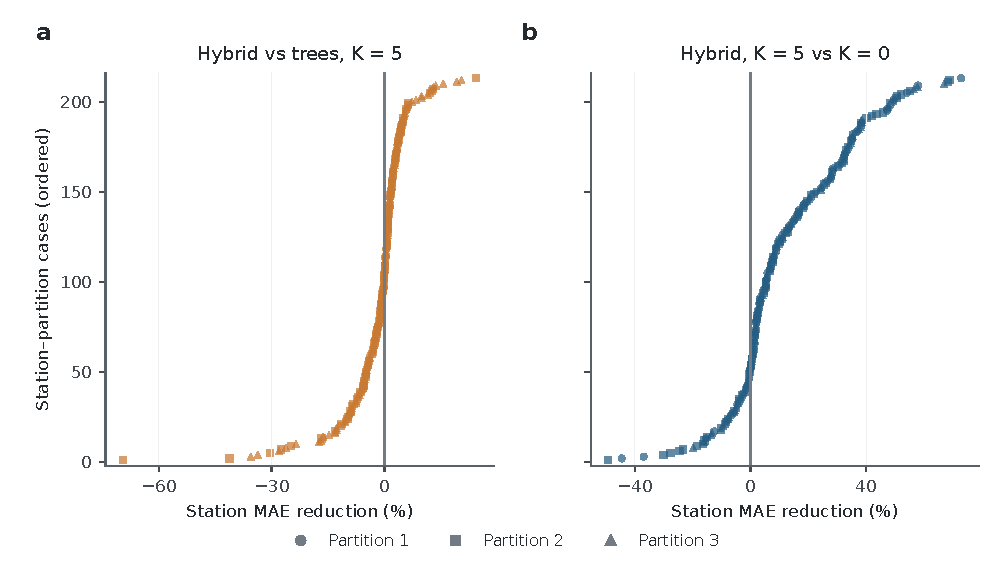
\includegraphics[width=\linewidth]{figures/unified_doc_station_responses.pdf}
\caption{\textbf{Station variation in reconstruction benefit.} \textbf{a,} Calibrated hybrid versus calibrated ExtraTrees at $K=5$. \textbf{b,} Calibrated hybrid versus its own $K=0$ prediction. Each point is a station--partition case; shapes identify the three partitions. Cases are ordered separately within each panel and do not align by station across panels. Positive values indicate lower MAE for the first predictor or $K=5$. Horizontal scales differ. The 213 cases represent 172 distinct test stations.}
\label{fig:unified_stations}
\end{figure}

\FloatBarrier
\section{Earlier regional station-calibration experiment}\label{app:regional}
\subsection{Regional prediction and support design}
We also examine whether sparse target observations can improve regional reconstruction at unmonitored stations. This experiment uses a separate regional ExtraTrees product with 120 trees and 40 source stations selected for each target by environmental similarity. Source descriptors combine hydroclimatic summaries, ecology, coordinates, and network attributes. Selection and descriptor scaling use available covariates, not target DOC labels. Its predictors include the visible DOC-context features described above.

At each of 43 target stations, five observed months are reserved as support candidates: the first, middle, last, first-quartile, and third-quartile positions of the observed record. Nested prefixes give $K=0,1,3,5$ support budgets. All five candidates are excluded from evaluation at every budget, leaving the same 2,316 query cells. A shrunken mean support residual adjusts the fixed regional prediction:
\begin{align}
 \bar r_i^{(K)}&=\frac{1}{K}\sum_{s\in\mathcal S_i^{(K)}}
       [z_{is}-\hat z_{is}^{\mathrm{reg}}],\\
 \hat y_{it}^{(K)}&=\max\{0,\exp(\hat z_{it}^{\mathrm{reg}}+
                      \alpha_K\bar r_i^{(K)})-1\}.
\end{align}
The correction is zero for $K=0$. The coefficients for $K=1,3,5$ are 0.25, 0.50, and 0.75, inherited unchanged from an earlier internal station-validation analysis. The base predictions remain fixed.

Support can follow a query month, and station descriptors summarize the available historical record. This extension evaluates retrospective station reconstruction. Its source-model configuration and query set differ from the main hybrid experiment; it evaluates sparse calibration rather than the performance of a jointly trained hybrid-plus-adapter model.


\subsection{Regional calibration results}
In the regional station-adaptation experiment, MAE decreases from 2.466~mg/L without target support to 2.320, 2.160, and 2.023~mg/L with one, three, and five observations per station (Table~\ref{tab:support}; Figure~\ref{fig:support}). Five observations yield a 17.9\% reduction on the unchanged query. The paired MAE difference is $-0.442$~mg/L, with a station-resampled 95\% interval of $[-1.026,-0.089]$~mg/L.

\begin{table}[htbp]\centering\small
\caption{Sparse station calibration in the separate regional experiment. Five seeds share 43 target stations and 2,316 fixed query cells. This baseline and query differ from Table~\ref{tab:main}.}
\label{tab:support}
% BEGIN GENERATED SUPPORT RESULTS
\begin{tabular}{rrrrr}\toprule
$K$ & MAE (mg/L) & Seed SD & RMSE (mg/L) & Reduction (\%)\\\midrule
0 & 2.466 & 0.007 & 5.390 & 0.00\\
1 & 2.320 & 0.013 & 4.968 & 5.90\\
3 & 2.160 & 0.011 & 4.746 & 12.41\\
5 & 2.023 & 0.008 & 4.412 & 17.93\\
\bottomrule\end{tabular}
% END GENERATED SUPPORT RESULTS
\end{table}

\begin{figure}[htbp]\centering
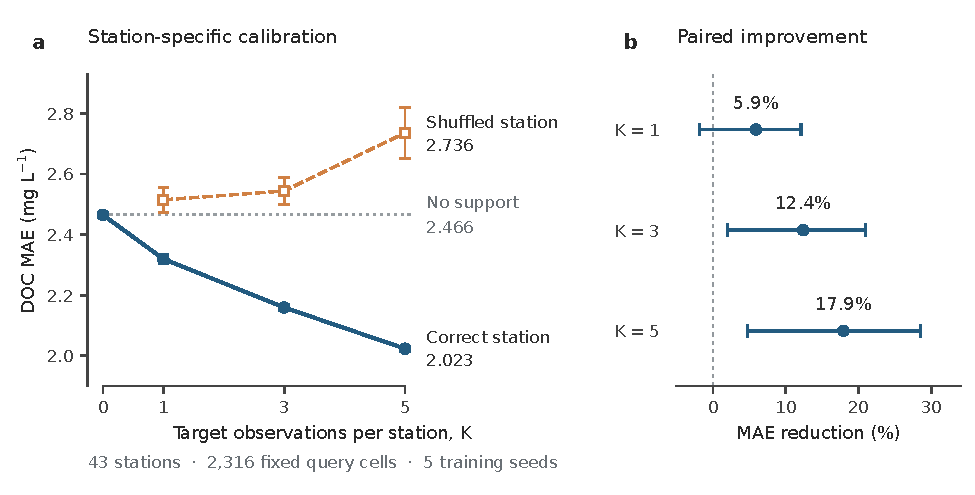
\includegraphics[width=\linewidth]{figures/doc_spatial_support_v2.pdf}
\caption{\textbf{Sparse target observations improve regional DOC reconstruction.} \textbf{a,} Mean DOC MAE across five training seeds as the number of observations per target station increases. The regional model and 2,316 query cells at 43 stations remain fixed. Correct-station calibration is compared with station-shuffled corrections and the uncalibrated reference; error bars show seed SD. Shuffling uses one fixed station permutation per seed and observation budget and serves as a descriptive diagnostic. \textbf{b,} Paired MAE reduction relative to no calibration, with 95\% station-bootstrap intervals preserving cell weighting. Support may occur after query months, so this experiment evaluates historical reconstruction.}
\label{fig:support}
\end{figure}

Calibration improves 36 of 43 stations. The median station-level relative reduction is 3.39\%, smaller than the pooled 17.9\%, indicating heterogeneous benefits and different weighting of station records (Figure~\ref{fig:station}). With five observations, assigning the station corrections to different targets increases mean MAE to 2.736~mg/L. This descriptive shuffle shows the importance of matching corrections to their own station; it does not identify the ecological cause of each station's bias.

\begin{figure}[htbp]\centering
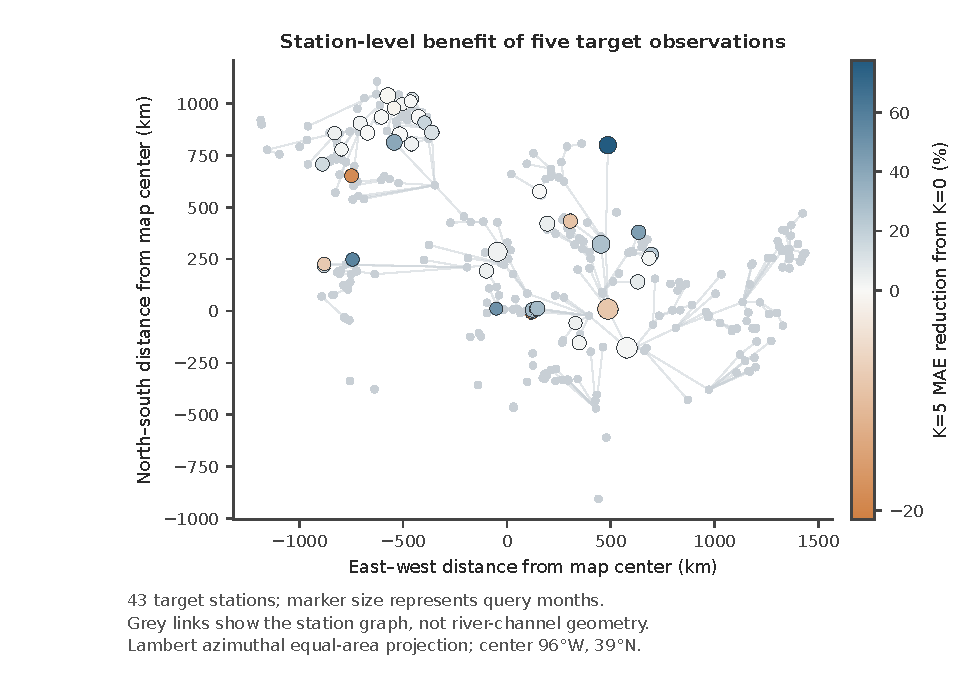
\includegraphics[width=\linewidth]{figures/doc_station_response_v2.pdf}
\caption{\textbf{Spatial heterogeneity in calibration benefit.} Five-observation station responses from the same regional product used in Table~\ref{tab:support}. Marker size represents the number of query months; color shows relative MAE reduction. The projected station coordinates are real; connecting lines represent graph links rather than mapped river-channel geometry.}
\label{fig:station}
\end{figure}


\FloatBarrier
\begin{thebibliography}{99}
\bibitem{yang2017}
Yang, Q., Zhang, X., Xu, X., and Asrar, G.~R. (2017).
An analysis of terrestrial and aquatic environmental controls of riverine dissolved organic carbon in the conterminous United States.
\emph{Water}, 9, 383.
\url{https://doi.org/10.3390/w9060383}.

\bibitem{tian2025}
Tian, S., Sha, A., Luo, Y., et al. (2025).
A novel framework for river organic carbon retrieval through satellite data and machine learning.
\emph{ISPRS Journal of Photogrammetry and Remote Sensing}, 221, 109--123.
\url{https://doi.org/10.1016/j.isprsjprs.2025.01.028}.

\bibitem{sterle2024}
Sterle, G., Perdrial, J., Kincaid, D.~W., et al. (2024).
CAMELS-Chem: augmenting CAMELS (Catchment Attributes and Meteorology for Large-sample Studies) with atmospheric and stream water chemistry data.
\emph{Hydrology and Earth System Sciences}, 28, 611--630.
\url{https://doi.org/10.5194/hess-28-611-2024}.

\bibitem{verhoef2006}
Ver Hoef, J.~M., Peterson, E., and Theobald, D. (2006).
Spatial statistical models that use flow and stream distance.
\emph{Environmental and Ecological Statistics}, 13, 449--464.
\url{https://doi.org/10.1007/s10651-006-0022-8}.

\bibitem{breiman2001}
Breiman, L. (2001).
Random forests.
\emph{Machine Learning}, 45, 5--32.
\url{https://doi.org/10.1023/A:1010933404324}.

\bibitem{geurts2006}
Geurts, P., Ernst, D., and Wehenkel, L. (2006).
Extremely randomized trees.
\emph{Machine Learning}, 63, 3--42.
\url{https://doi.org/10.1007/s10994-006-6226-1}.

\bibitem{cini2022}
Cini, A., Marisca, I., and Alippi, C. (2022).
Filling the G\_ap\_s: multivariate time series imputation by graph neural networks.
\emph{International Conference on Learning Representations}.
\url{https://openreview.net/forum?id=kOu3-S3wJ7}.

\bibitem{che2018}
Che, Z., Purushotham, S., Cho, K., Sontag, D., and Liu, Y. (2018).
Recurrent neural networks for multivariate time series with missing values.
\emph{Scientific Reports}, 8, 6085.
\url{https://doi.org/10.1038/s41598-018-24271-9}.

\bibitem{roberts2017}
Roberts, D.~R., Bahn, V., Ciuti, S., et al. (2017).
Cross-validation strategies for data with temporal, spatial, hierarchical, or phylogenetic structure.
\emph{Ecography}, 40, 913--929.
\url{https://doi.org/10.1111/ecog.02881}.
\end{thebibliography}
\end{document}
